

\documentclass[spanish, a4paper, 12pt]{article} 	%idioma, tamaño, tamaño letra, tipo de documento (articulo, libro, report)
\usepackage[english, activeacute]{babel}		%babel para tildes: á = \´{a}	
\usepackage[utf8]{inputenc}
\usepackage{geometry}
\usepackage{multicol}
\usepackage{amsmath}
\usepackage{amssymb}
%\usepackage{amsttthm}
\usepackage{graphics}
\usepackage{graphicx}
\usepackage{hyperref}

\usepackage{fancyhdr}
\geometry{a4paper, textwidth=16cm, textheight=20cm}
\pagestyle{fancy}
%\usepackage{nicefrac}
%\setlenght{\parskip}{1}
\lhead{Métodos algorítmicos}
\cfoot{\thepage}
\renewcommand{\headrulewidth}{0.4pt}
\renewcommand{\footrulewidth}{0.4pt}

\begin{document}
\title{\textbf{Inteligencia Artificial}}
\maketitle


\center{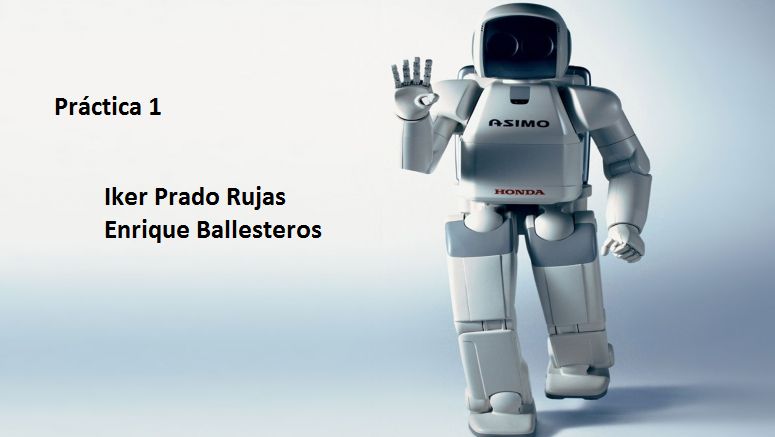
\includegraphics[width=\textwidth]{robotHonda.png}}

\newpage
\textbf{{¿Qué es la inteligencia artificial?}}


\begin{section}
	%\begin{section}{Irene}
	Básicamente solo es capaz de analizar frases sencillas, con una estructura concreta y siempre relacionadas con su campo.
	 Aunque también te saluda y se aprende tu nombre. Es más práctico buscar tú los billetes o usar un buscador porque 
	 cuando le preguntas sobre el billete más barato o el tren más rápido no sabe ayudarte.
	 Tiene una guía de uso pero es demasiado optimista creemos: \url{www.renfe.com/empresa/ayudav.html}
	 
	%\end{section}
	%\begin{section}{Anna}
	
	Resumo su funcionamiento en esta conversación:
	
	-Anna ha dicho: Hola, soy Anna, asistente virtual de IKEA. Estoy aquí para ayudarte a mejorar tu experiencia con la página 		web de IKEA, productos y servicios. Hazme una pregunta, y yo te proporcionaré la respuesta más apropiada. 
¿Cómo funciono? Siempre trata de escribir frases cortas, y sólo una a la vez. Cuanto más larga sea tu pregunta, la posibilidad de darte una respuesta incorrecta incrementará. A veces abro una página web con información referente a tu pregunta y mis respuestas pueden tener enlaces en las que puedes pulsar, si lo haces llegarás a respuestas adicionales, con información relacionada. Me encanta aprender, así que si tu pregunta no está en mi base de datos, voy a solicitar que se la agregue a mi conocimiento, tan pronto como sea posible. Tus comentarios serán muy apreciados! Ahora vamos a tener una charla, ¿de acuerdo?
	+Has dicho: De acuerdo.
	-Anna ha dicho: Lo siento, no he entendido bien lo que has dicho.
	
	Con esto basta para darse cuenta que está lejos de poder ser denominado inteligencia artificial.
	%\end{section}
	%\begin{section}
		Alice
		
		Realmente de las cuatro es la única que puede considerarse inteligencia artificial.
	%\end{section}
	%\begin{section}
		Eliza
		
	Realmente si necesitas alguien que te escuche y se interese por tus problemas resulta un bot muy interesante. Pero si intentas que razone mínimamente y que te responda puedes ir olvidándote. A preguntas tan sencillas como  \textit{¿Cuántos años tienes ?} no es capaz de responder y sencillamente te suelta una de sus respuestas predeterminada quizá cambiando la conjugación de algún verbo. Por ello como inteligencia artificial no tiene mucho sentido dedicarle más tiempo.
	
	%\end{section}
\end{section}
\begin{section}{Deep Blue y Walter}
	Deep blue es una supercomputadora fabricada en los años 60 por IBM desarrollada para jugar al ajedrez, que en 1996 se enfrentó al campeón del mundo Gary Kaspárov. Consiguió vencerle una vez, pero al mejor de 6 Deep Blue fue vencido.
	
	Más tarde, una versión mejorada de Deep Blue, consiguió vencer a Kaspárov ajustadamente en un encuentro a 6 partidas. Aún así Kaspárov denunció irregularidades en estas partidas que nunca llegaron a ser explicadas por IBM. 
	
	La limitación de Deep Blue, realmente es la limitación que encuentran todas las máquinas que intentan jugar al ajedrez. El espacio de estados es enorme debido a la complejidad del juego, por lo que es imposible explorar todas las opciones hasta el final. Lo que hizo diferente a Deep Blue, además del bombo que le dio IBM que lo usó de escaparate para su empresa, fue que contaba con 30  microprocesadores y 480 procesadores especializados en el ajedrez. Sencillamente fue la máquina más potente que se dedicó al ajedrez en la época por lo que logró los mejores resultados. Era capaz de calcular 200 posiciones por segundo, que aunque daba una exploración limitada, dedicando suficiente tiempo era capaz de plantar cara al campeón del mundo.
	
	
	
	Watson es un sistema informático de inteligencia artificial desarrollado por IBM diseñado para ser capaz de responder preguntas realizadas en lenguaje natural.
	
	Es famoso porque fue capaz de derrotar en el concurso televisivo \textit{Jeopardy!} al que más dinero había ganado en la historia del concurso y al que más programas seguidos había estado.
	
	Su principal limitación está en el tiempo que necesita para ser capaz de procesar una pregunta y responderla. Aun así fue capaz de vencer en el concurso gracias a la ejecución de miles de algoritmos distintos para la misma pregunta, lo que le permitía elegir la respuesta que más algoritmos encontrasen a la vez que cotejaba en su base de datos si la respuesta tenía sentido, y de esta forma aumentar la probabilidad de acierto para una respuesta dada. 
\end{section}

\end{document}

